\section{Technical Approach}
To infer information about Java code we use existing inference tools and
combine their output. We have additionally developed a simple framework to aid
in writing our own analyses, should that prove necessary.

To combine the results of disparate analyses we have to convert their results
into a common format at some point in our toolchain.  We will use the JAIF
(Java Annotation Index File) format for that purpose.  Some anaylses generate
results directly in JAIF format, some provide annotated bytecodes which can be
easily extracted into JAIF format, and others provide textual results for which
we will write simple translators into JAIF format.

\begin{figure}
\centering
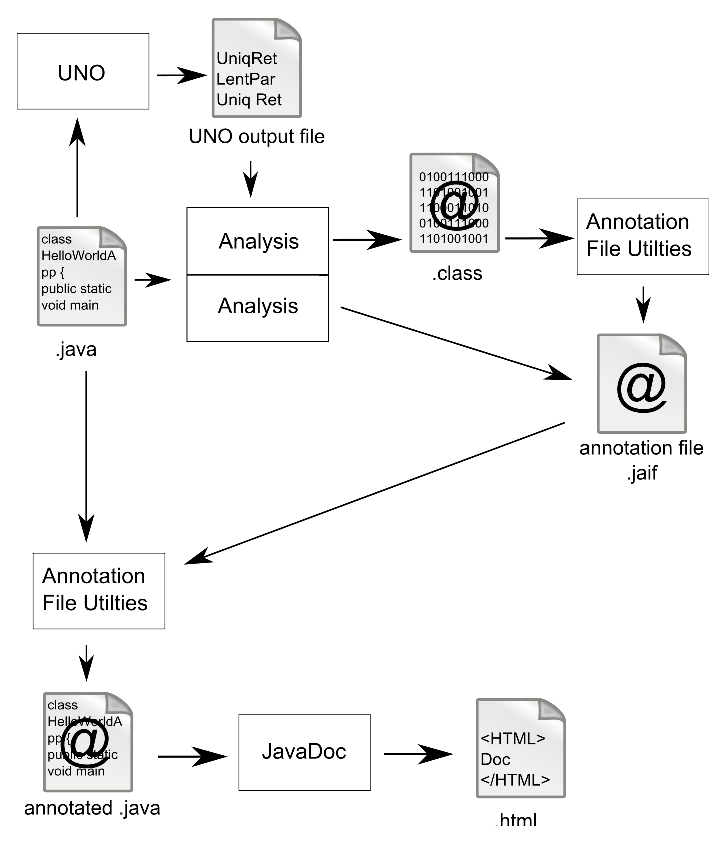
\psfig{file=figures/technicalApproach/technicalApproach.eps, width=3in}
\caption{Toolchain}
\label{fig:toolchain}
\end{figure}

In the following section we describe our simple analysis framework.  In
sections~\ref{sec:Javarifier} through~\ref{sec:Nullability} we describe each of
the existing analyses we will be using in our evaluation and how we will
integrate its results into our toolchain. In the section~\ref{sec:jaif2html} we
explain the final step of our process which is to integrate the various
analysis into the Javadoc generation process.

Figure \ref{fig:toolchain} shows the stages in our toolchain.

\subsection{Analysis Framework}
\label{ss:analysisFramework}

To implement our own analysis tools we use the Annotation Processing Tool (APT)
API~\cite{apt} built into the Java standard compiler.  From within an APT plugin
we can access the compiler's abstract syntax tree and augment the generated
bytecode with annotations representing our analysis results. These annotations
are then extracted into external annotation files.

\subsection{Javarifier}
\label{sec:Javarifier}

Javarifier is a tool to infer reference immutability information built in
conjuction with research done by Quinonez et al.~\cite{Javarifier}. It infers
mutability constraints for object fields, method arguments and receivers. Those
constraints may be \texttt{mutable}, \texttt{readonly}, \texttt{?~readonly},
\texttt{polyread}, and \texttt{this-mutable}. The \texttt{?~readonly}
constraint indicates a method argument with a \texttt{readonly} upper bound and
a \texttt{mutable} lower bound. The \texttt{polyread} constraint provides
polymorphism over mutability for method arguments and receivers
(i.e. indicating that a method is read-only when called through a read-only
reference or mutable when called through a mutable reference). A
\texttt{this-mutable} reference provides similar polymorphism for object
fields: a \texttt{this-mutable} field is mutable if \texttt{this} is mutable
and read-only otherwise.

Javarifier produces its results directly in the JAIF format which allows us to
easily integrate it into our toolchain. We need simply to express the meaning
of its inferred constraints in the Javadoc documentation in concise language.

\subsection{Uno}

Uno is an open source tool which is the outcome of research done by Ma and
Foster~\cite{Uno}. It infers alias and encapsulation properties for Java.  The
tool generates annotations which provide information about how a certain
function treats its parameters, return values and fields (in the case of a
non-static function) when called. E.g. if a function captures or leaks a
reference or returns a new unique reference.

The tool generates annotations which are stored in a single separate file. 
To integrate the analysis results of UNO into the Java documentation we
use our own framework. We implemented a tree visitor inside the Java 7 
compiler that, at initialization, reads in the file generated by UNO and 
stores the information in a hashset. During the iteration over the AST
our visitor inserts annotation at the appropriate places.

\subsection{Thrown Exceptions}

Java requires that checked exceptions be declared by methods that raise them,
but it unfortunately cannot require that they be well documented, and
frequently the conditions under which exceptions are raised are unclear to a
library user. Additionally, unchecked exceptions need not be declared in method
signatures nor documentation and can remain entirely invisible to the library
user until they are encountered at runtime.

Buse and Weimer infer documentation for the conditions that cause some
exceptions~\cite{autodoc}.  Their analysis locates explicit throws of
exceptions and performs some symbolic execution along with propagating results
between methods to determine exceptional input conditions.  We do not use an
existing analysis tool for this purpose, as none were available.  Our analysis
is a fairly simple search for explicit throws, tracking branch statements on the
way to such statements and propagating some information about thrown runtime
(unchecked) exceptions between methods.

\subsection{Nullability}
\label{sec:Nullability}

In heavily object oriented languages like java, every variable is nullable
(aka. option, maybe), capable of holding either a reference to a value or the
special value null.  Because of this ubiquity, one common mistake is to call
methods with null parameters they are unprepared to handle, or to erroneously
assume that returned values are never null.  Well documented libraries, like
the Java collections framework, will frequently spell out when variables are
assumed to be nullable or not-null when an ambiguity seems likely.

By means of a nullability inference~\cite{NIT,NonNullTypeInference} we can add
similarly useful type decorations to documentation.  Although two Java
nullability inferences are freely available, they are both whole program
analyses and therefore ill-suited to our target application: library
documentation.  We plan to first try adapting their existing analysis code, or
failing that re-implement a modular version of their analysis within our own
framework.

\subsection{From JAIF to HTML documentation}
\label{sec:jaif2html}

Once the results of the various analyses have been collected into a set of
annotation files, we use the annotation file utilities~\cite{AFU} to merge
those annotations back into the original library source. We then use a custom
Javadoc doclet~\cite{doclet} to augment the original Javadoc documentation (if
any) with the information represented by the analysis annotations.

For each analysis, we provide a mapping from the annotation data to either a
textual or iconic representation of the constraints it describes. For example,
a method parameter annotated with \texttt{@Nullable} may result in the text
``(null allowed)'' being appended to the documentation for that parameter. We
will also investigate representing very common annotations such as nullability
in a compact iconic form to avoid overwhelming any existing documentation with
our analysis-derived additions.
